\newpage
\newcommand{\SubItem}[1]{
    {\setlength\itemindent{15pt} \item[-] #1}
}

\section{Google Groups}\index{Google Groups}
Google Groups is a great forum for asynchronous communication with students. I find that it is more user friendly than Blackboard's native discussion group features.  When embedded in Blackboard, students can access a course-specific discussion board with just a single click!  Groups are highly configurable, easily searched, and organization of discussions is under the control of the account owner.

In order to set up a Google Group:
\begin{enumerate}
    \item Visit \weblink{https://groups.google.com} and log in with your W\&M credentials.
    \item Click ``Create group"
    \item Enter a name/description for your group and select the options that will determine which features are available in your group (see Figure \ref{fig:googlegroup1}).\\
    \textit{Note: I prefer to use the ``Q\&A forum" option as the format for my class discussion groups because it includes some nice features like allowing students to ``vote" up or down on existing posts/questions and the ability to mark items ``resolved".}
    \begin{figure}[ht]
    \centering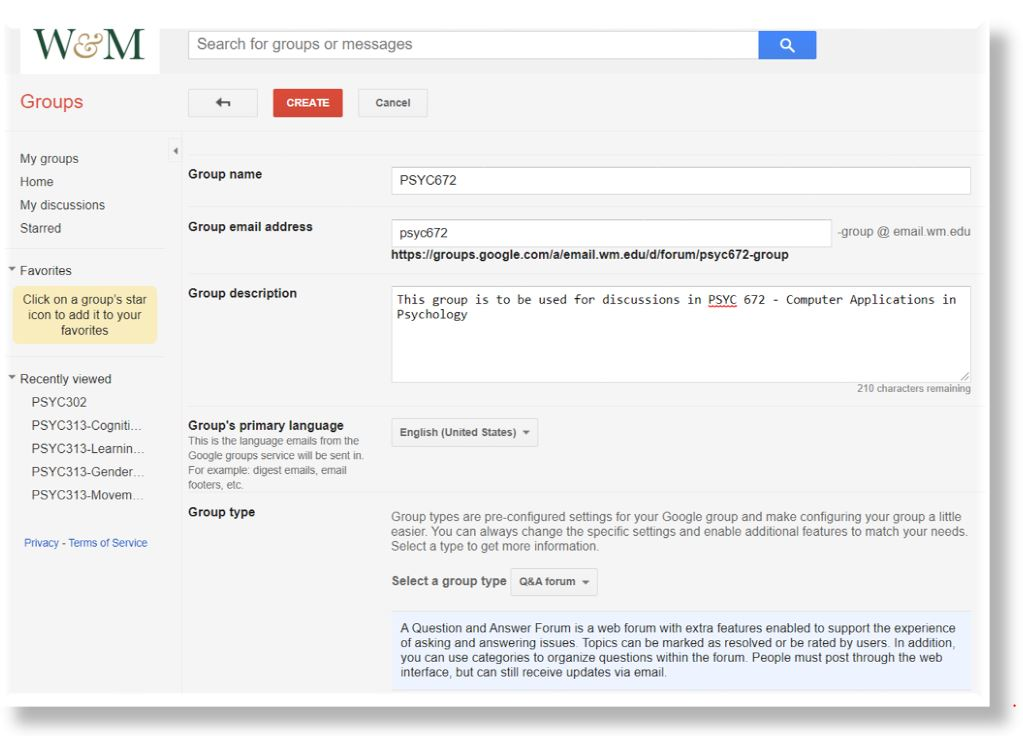
\includegraphics[scale=0.6]{googlegroups1.JPG}
    \caption{Creating a Google Group}
    \label{fig:googlegroup1}
    \end{figure}
    
    \item Scroll down and set your basic visibility and access settings, then click ``Create" to initialize the group.
    \newpage
    \item Get the address of your new group from the address bar in your browser (see Figure \ref{fig:googlegroups2}). You will need this to embed the group in Blackboard.
    \begin{figure}[h]
    \centering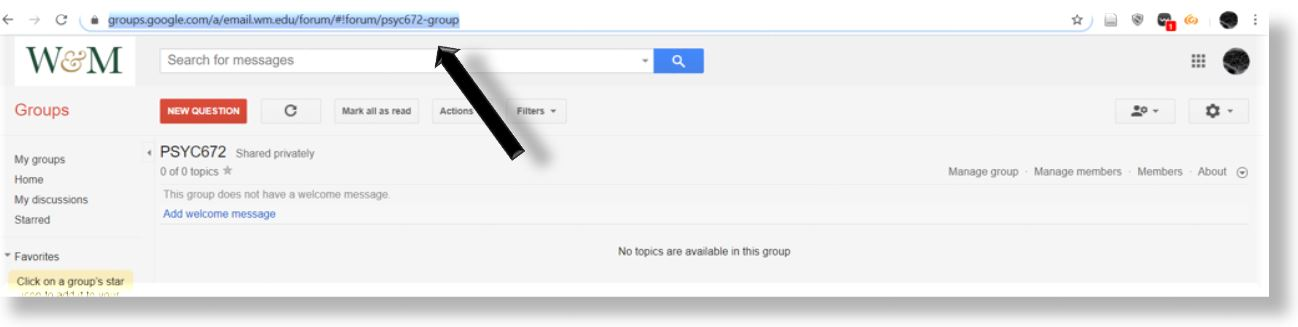
\includegraphics[scale=0.5]{googlegroups2.JPG}
    \caption{A new Google group}
    \label{fig:googlegroups2}
    \end{figure}
    
    \item Embed the group in Blackboard.
    \SubItem If you don't have one already, create a new content area to hold the group.
    \begin{figure}[h]
    \centering
    \centering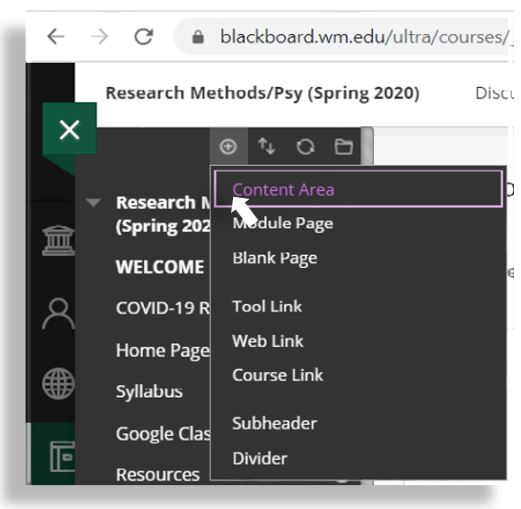
\includegraphics[scale=0.5]{googlegroups3.JPG}
    \caption{Zoom profile}
    \label{fig:googlegroups3}
    \end{figure}
    
    \SubItem Next, add a new ``Item" your content area in Blackboard.
    \begin{figure}[h]
    \centering
    \centering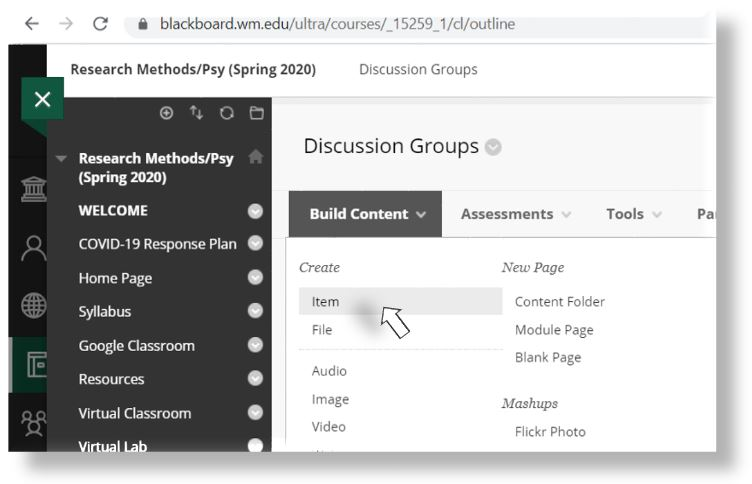
\includegraphics[scale=0.5]{googlegroups4.JPG}
    \caption{Zoom profile}
    \label{fig:googlegroups4}
    \end{figure}
    
    \SubItem Click the ``HTML" button in the text editor panel (see Figure \ref{fig:googlegroups5}) to open the HTML window.
    \begin{figure}[h]
    \centering
    \centering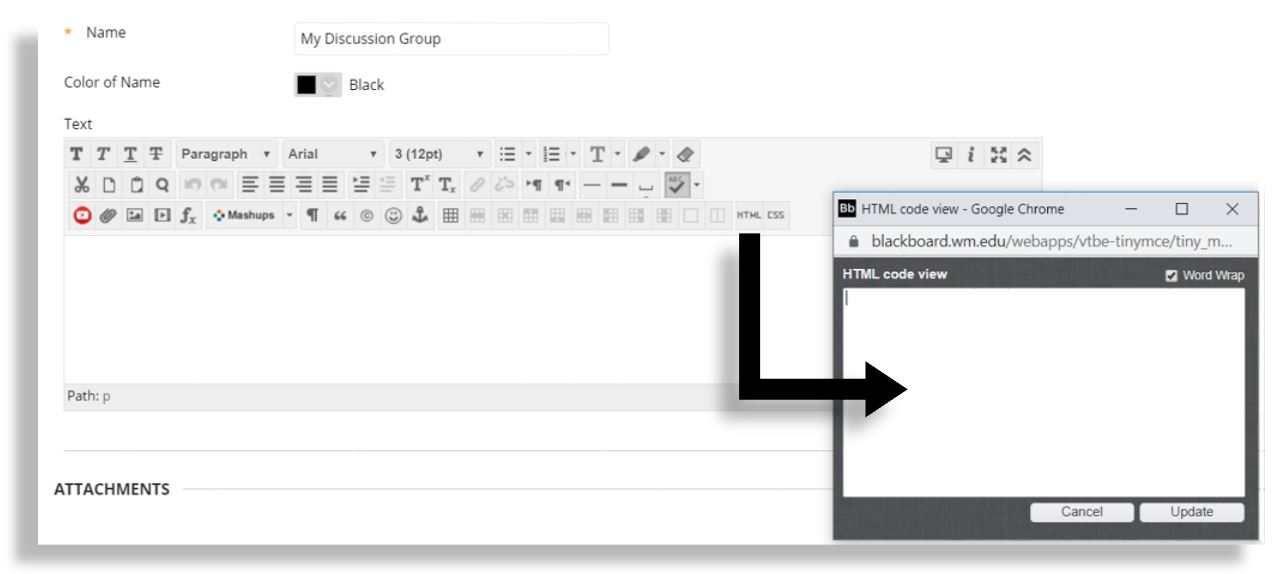
\includegraphics[scale=0.5]{googlegroups5.JPG}
    \caption{Embedding the group}
    \label{fig:googlegroups5}
    \end{figure}
    
    \SubItem Now go to your Google Groups group page and click the settings (gear icon) button and select ``group settings".
    
    \SubItem Scroll down until you see ``Embedding your group", then copy the embed code provided for you. 

    \SubItem Paste the code you just copied into the HTML window in Blackboard and click the ``Update" button. A yellow box will appear in the text panel of the Blackboard item.  Click the ``Submit" button to complete the process.
\end{enumerate} 
\vspace{.5cm}

Once these steps are completed, your students will be able to access the discussion board with a single click on the Content Area in Blackboard.  Students can easily post a new question, or search/filter existing posts for answers to previously posted questions (see Figure \ref{fig:googlegroups6}).
    \begin{figure}[h]
    \centering
    \centering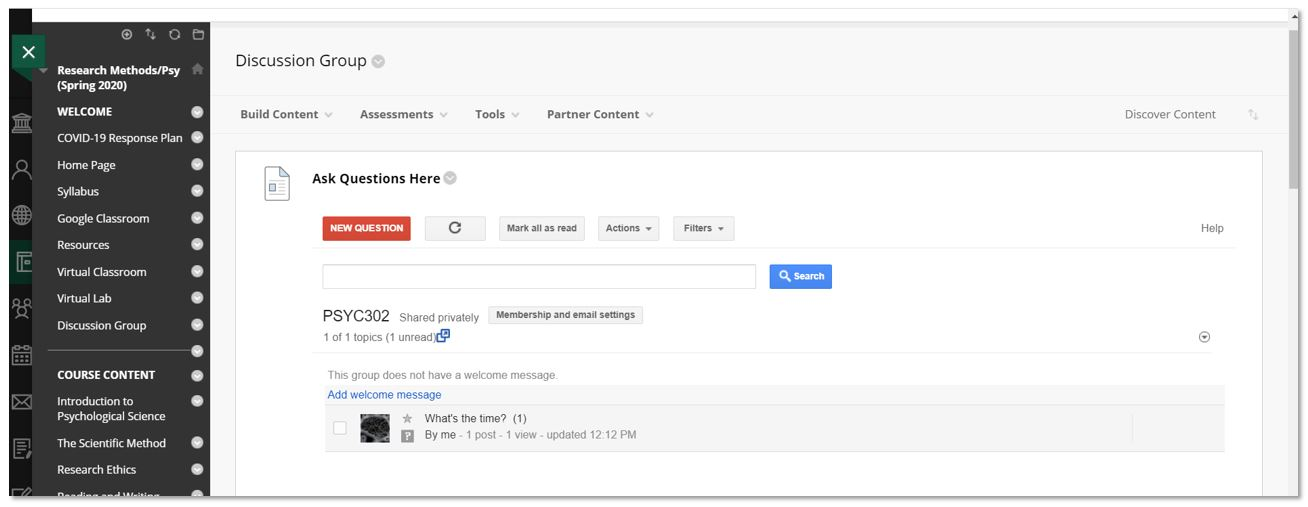
\includegraphics[scale=0.55]{googlegroups6.JPG}
    \caption{Google Group embedded in Blackboard}
    \label{fig:googlegroups6}
    \end{figure}
%\begin{lstlisting}[language=HTML,basicstyle=\footnotesize]
